\documentclass[english,dit,thesis]{hogentreport}

\usepackage{lipsum} % For blind text, can be removed after adding actual content

%% Pictures to include in the text can be put in the graphics/ folder
\graphicspath{{graphics/}}

%% For source code highlighting, requires pygments to be installed
%% Compile with the -shell-escape flag!
\usepackage[section]{minted}

\usemintedstyle{solarized-light}
\definecolor{bg}{RGB}{253,246,227} %% Set the background color of the codeframe

%% Change this line to edit the line numbering style:
\renewcommand{\theFancyVerbLine}{\ttfamily\scriptsize\arabic{FancyVerbLine}}

%% Macro definition to load external java source files with \javacode{filename}:
\newmintedfile[javacode]{java}{
    bgcolor=bg,
    fontfamily=tt,
    linenos=true,
    numberblanklines=true,
    numbersep=5pt,
    gobble=0,
    framesep=2mm,
    funcnamehighlighting=true,
    tabsize=4,
    obeytabs=false,
    breaklines=true,
    mathescape=false
    samepage=false,
    showspaces=false,
    showtabs =false,
    texcl=false,
}

% Other packages not already included can be imported here

%%---------- Document metadata -------------------------------------------------
% TODO: Replace this with your own information
\author{Robbe Cherlet}
\supervisor{Mevr. C. Teerlinck}
\cosupervisor{Dhr. J. Delamper}
\title[A Comparative Analysis and Proof of Concept]%
    {Sustainability in Continuous Integration en Deployment-processes}
\academicyear{\advance\year by -1 \the\year--\advance\year by 1 \the\year}
\examperiod{1}
\degreesought{\IfLanguageName{dutch}{Professionele bachelor in de toegepaste informatica}{Bachelor of applied computer science}}
\partialthesis{false} %% To display 'in partial fulfilment'
%\institution{Internshipcompany BVBA.}

%% Add global exceptions to the hyphenation here
\hyphenation{back-slash}

%% The bibliography (style and settings are  found in hogentthesis.cls)
\addbibresource{bachproef.bib}            %% Bibliography file
\addbibresource{../voorstel/voorstel.bib} %% Bibliography research proposal
\defbibheading{bibempty}{}

%% Prevent empty pages for right-handed chapter starts in twoside mode
\renewcommand{\cleardoublepage}{\clearpage}

\renewcommand{\arraystretch}{1.2}

%% Content starts here.
\begin{document}

%---------- Front matter -------------------------------------------------------

\frontmatter

\hypersetup{pageanchor=false} %% Disable page numbering references
%% Render a Dutch outer title page if the main language is English
\IfLanguageName{english}{%
    %% If necessary, information can be changed here
    \degreesought{Professionele Bachelor toegepaste informatica}%
    \begin{otherlanguage}{dutch}%
       \maketitle%
    \end{otherlanguage}%
}{}

%% Generates title page content
\maketitle
\hypersetup{pageanchor=true}

%%=============================================================================
%% Voorwoord
%%=============================================================================

\chapter*{\IfLanguageName{dutch}{Woord vooraf}{Preface}}%
\label{ch:voorwoord}

%% TODO:
%% Het voorwoord is het enige deel van de bachelorproef waar je vanuit je
%% eigen standpunt (``ik-vorm'') mag schrijven. Je kan hier bv. motiveren
%% waarom jij het onderwerp wil bespreken.
%% Vergeet ook niet te bedanken wie je geholpen/gesteund/... heeft



test commit

\lipsum[1-2]
%%=============================================================================
%% Samenvatting
%%=============================================================================

% TODO: De "abstract" of samenvatting is een kernachtige (~ 1 blz. voor een
% thesis) synthese van het document.
%
% Een goede abstract biedt een kernachtig antwoord op volgende vragen:
%
% 1. Waarover gaat de bachelorproef?
% 2. Waarom heb je er over geschreven?
% 3. Hoe heb je het onderzoek uitgevoerd?
% 4. Wat waren de resultaten? Wat blijkt uit je onderzoek?
% 5. Wat betekenen je resultaten? Wat is de relevantie voor het werkveld?
%
% Daarom bestaat een abstract uit volgende componenten:
%
% - inleiding + kaderen thema
% - probleemstelling
% - (centrale) onderzoeksvraag
% - onderzoeksdoelstelling
% - methodologie
% - resultaten (beperk tot de belangrijkste, relevant voor de onderzoeksvraag)
% - conclusies, aanbevelingen, beperkingen
%
% LET OP! Een samenvatting is GEEN voorwoord!

%%---------- Nederlandse samenvatting -----------------------------------------
%
% TODO: Als je je bachelorproef in het Engels schrijft, moet je eerst een
% Nederlandse samenvatting invoegen. Haal daarvoor onderstaande code uit
% commentaar.
% Wie zijn bachelorproef in het Nederlands schrijft, kan dit negeren, de inhoud
% wordt niet in het document ingevoegd.

\IfLanguageName{english}{%
\selectlanguage{dutch}
\chapter*{Samenvatting}
\lipsum[1-4]
\selectlanguage{english}
}{}

%%---------- Samenvatting -----------------------------------------------------
% De samenvatting in de hoofdtaal van het document

\chapter*{\IfLanguageName{dutch}{Samenvatting}{Abstract}}

\lipsum[1-4]


%---------- Inhoud, lijst figuren, ... -----------------------------------------

\tableofcontents

% In a list of figures, the complete caption will be included. To prevent this,
% ALWAYS add a short description in the caption!
%
%  \caption[short description]{elaborate description}
%
% If you do, only the short description will be used in the list of figures

\listoffigures

% If you included tables and/or source code listings, uncomment the appropriate
% lines.
%\listoftables
%\listoflistings

% Als je een lijst van afkortingen of termen wil toevoegen, dan hoort die
% hier thuis. Gebruik bijvoorbeeld de ``glossaries'' package.
% https://www.overleaf.com/learn/latex/Glossaries

%---------- Kern ---------------------------------------------------------------

\mainmatter{}

% De eerste hoofdstukken van een bachelorproef zijn meestal een inleiding op
% het onderwerp, literatuurstudie en verantwoording methodologie.
% Aarzel niet om een meer beschrijvende titel aan deze hoofdstukken te geven of
% om bijvoorbeeld de inleiding en/of stand van zaken over meerdere hoofdstukken
% te verspreiden!

%%=============================================================================
%% Inleiding
%%=============================================================================

\chapter{\IfLanguageName{dutch}{Inleiding}{Introduction}}%
\label{ch:inleiding}

De inleiding moet de lezer net genoeg informatie verschaffen om het onderwerp te begrijpen en in te zien waarom de onderzoeksvraag de moeite waard is om te onderzoeken. In de inleiding ga je literatuurverwijzingen beperken, zodat de tekst vlot leesbaar blijft. Je kan de inleiding verder onderverdelen in secties als dit de tekst verduidelijkt. Zaken die aan bod kunnen komen in de inleiding~\autocite{Pollefliet2011}:

\begin{itemize}
  \item context, achtergrond
  \item afbakenen van het onderwerp
  \item verantwoording van het onderwerp, methodologie
  \item probleemstelling
  \item onderzoeksdoelstelling
  \item onderzoeksvraag
  \item \ldots
\end{itemize}

\section{\IfLanguageName{dutch}{Probleemstelling}{Problem Statement}}%
\label{sec:probleemstelling}

Uit je probleemstelling moet duidelijk zijn dat je onderzoek een meerwaarde heeft voor een concrete doelgroep. De doelgroep moet goed gedefinieerd en afgelijnd zijn. Doelgroepen als ``bedrijven,'' ``KMO's'', systeembeheerders, enz.~zijn nog te vaag. Als je een lijstje kan maken van de personen/organisaties die een meerwaarde zullen vinden in deze bachelorproef (dit is eigenlijk je steekproefkader), dan is dat een indicatie dat de doelgroep goed gedefinieerd is. Dit kan een enkel bedrijf zijn of zelfs één persoon (je co-promotor/opdrachtgever).

\section{\IfLanguageName{dutch}{Onderzoeksvraag}{Research question}}%
\label{sec:onderzoeksvraag}

Wees zo concreet mogelijk bij het formuleren van je onderzoeksvraag. Een onderzoeksvraag is trouwens iets waar nog niemand op dit moment een antwoord heeft (voor zover je kan nagaan). Het opzoeken van bestaande informatie (bv. ``welke tools bestaan er voor deze toepassing?'') is dus geen onderzoeksvraag. Je kan de onderzoeksvraag verder specifiëren in deelvragen. Bv.~als je onderzoek gaat over performantiemetingen, dan 

\section{\IfLanguageName{dutch}{Onderzoeksdoelstelling}{Research objective}}%
\label{sec:onderzoeksdoelstelling}

Wat is het beoogde resultaat van je bachelorproef? Wat zijn de criteria voor succes? Beschrijf die zo concreet mogelijk. Gaat het bv.\ om een proof-of-concept, een prototype, een verslag met aanbevelingen, een vergelijkende studie, enz.

\section{\IfLanguageName{dutch}{Opzet van deze bachelorproef}{Structure of this bachelor thesis}}%
\label{sec:opzet-bachelorproef}

% Het is gebruikelijk aan het einde van de inleiding een overzicht te
% geven van de opbouw van de rest van de tekst. Deze sectie bevat al een aanzet
% die je kan aanvullen/aanpassen in functie van je eigen tekst.

De rest van deze bachelorproef is als volgt opgebouwd:

In Hoofdstuk~\ref{ch:stand-van-zaken} wordt een overzicht gegeven van de stand van zaken binnen het onderzoeksdomein, op basis van een literatuurstudie.

In Hoofdstuk~\ref{ch:methodologie} wordt de methodologie toegelicht en worden de gebruikte onderzoekstechnieken besproken om een antwoord te kunnen formuleren op de onderzoeksvragen.

% TODO: Vul hier aan voor je eigen hoofstukken, één of twee zinnen per hoofdstuk

In Hoofdstuk~\ref{ch:conclusie}, tenslotte, wordt de conclusie gegeven en een antwoord geformuleerd op de onderzoeksvragen. Daarbij wordt ook een aanzet gegeven voor toekomstig onderzoek binnen dit domein.
\chapter{\IfLanguageName{dutch}{Stand van zaken}{State of the art}}%
\label{ch:stand-van-zaken}

% Tip: Begin elk hoofdstuk met een paragraaf inleiding die beschrijft hoe
% dit hoofdstuk past binnen het geheel van de bachelorproef. Geef in het
% bijzonder aan wat de link is met het vorige en volgende hoofdstuk.

% Pas na deze inleidende paragraaf komt de eerste sectiehoofding.

Dit hoofdstuk bevat je literatuurstudie. De inhoud gaat verder op de inleiding, maar zal het onderwerp van de bachelorproef *diepgaand* uitspitten. De bedoeling is dat de lezer na lezing van dit hoofdstuk helemaal op de hoogte is van de huidige stand van zaken (state-of-the-art) in het onderzoeksdomein. Iemand die niet vertrouwd is met het onderwerp, weet nu voldoende om de rest van het verhaal te kunnen volgen, zonder dat die er nog andere informatie moet over opzoeken \autocite{Pollefliet2011}.

Je verwijst bij elke bewering die je doet, vakterm die je introduceert, enz.\ naar je bronnen. In \LaTeX{} kan dat met het commando \texttt{$\backslash${textcite\{\}}} of \texttt{$\backslash${autocite\{\}}}. Als argument van het commando geef je de ``sleutel'' van een ``record'' in een bibliografische databank in het Bib\LaTeX{}-formaat (een tekstbestand). Als je expliciet naar de auteur verwijst in de zin (narratieve referentie), gebruik je \texttt{$\backslash${}textcite\{\}}. Soms is de auteursnaam niet expliciet een onderdeel van de zin, dan gebruik je \texttt{$\backslash${}autocite\{\}} (referentie tussen haakjes). Dit gebruik je bv.~bij een citaat, of om in het bijschrift van een overgenomen afbeelding, broncode, tabel, enz. te verwijzen naar de bron. In de volgende paragraaf een voorbeeld van elk.

\textcite{Knuth1998} schreef een van de standaardwerken over sorteer- en zoekalgoritmen. Experten zijn het erover eens dat cloud computing een interessante opportuniteit vormen, zowel voor gebruikers als voor dienstverleners op vlak van informatietechnologie~\autocite{Creeger2009}.

Let er ook op: het \texttt{cite}-commando voor de punt, dus binnen de zin. Je verwijst meteen naar een bron in de eerste zin die erop gebaseerd is, dus niet pas op het einde van een paragraaf.

\lipsum[7-20]

%%=============================================================================
%% Methodologie
%%=============================================================================

\chapter{\IfLanguageName{dutch}{Methodologie}{Methodology}}%
\label{ch:methodologie}

%% TODO: In dit hoofstuk geef je een korte toelichting over hoe je te werk bent
%% gegaan. Verdeel je onderzoek in grote fasen, en licht in elke fase toe wat
%% de doelstelling was, welke deliverables daar uit gekomen zijn, en welke
%% onderzoeksmethoden je daarbij toegepast hebt. Verantwoord waarom je
%% op deze manier te werk gegaan bent.
%% 
%% Voorbeelden van zulke fasen zijn: literatuurstudie, opstellen van een
%% requirements-analyse, opstellen long-list (bij vergelijkende studie),
%% selectie van geschikte tools (bij vergelijkende studie, "short-list"),
%% opzetten testopstelling/PoC, uitvoeren testen en verzamelen
%% van resultaten, analyse van resultaten, ...
%%
%% !!!!! LET OP !!!!!
%%
%% Het is uitdrukkelijk NIET de bedoeling dat je het grootste deel van de corpus
%% van je bachelorproef in dit hoofstuk verwerkt! Dit hoofdstuk is eerder een
%% kort overzicht van je plan van aanpak.
%%
%% Maak voor elke fase (behalve het literatuuronderzoek) een NIEUW HOOFDSTUK aan
%% en geef het een gepaste titel.

\section{Phase 1: Literary review}
The research will be divided into 4 phases, the first of which is a literature review. This will be performed to examine existing approaches and gain deeper insights into the evolution of CI/CD practices.

\section{Phase 2: Metrics and Tools Analysis}
This phase will delve into the design of the research, focusing on the methodology and the approach taken to address the research questions. The chapter will also provide an overview of the research design, the research methods, and the data collection techniques used to address the research questions.

\section{Phase 3: Case Study}
The subsequent phase of the bachelor thesis involves a case study at Wolters Kluwer to evaluate the environmental impact of the current CI/CD practices. This case study will provide insight into the environmental impact by analyzing the energy consumption, carbon footprint, and resource utilization of the CI/CD practices at Wolters Kluwer. Additionally, the case study will evaluate the efficiency and scalability of these CI/CD practices.

\section{Phase 4: Comparative Study}
The fourth phase of the research will involve a comparative study between Windows and Linux agents. This phase will compare the energy-efficiency and performance of Windows and Linux agents in a TeamCity instance. 

\section{Phase 5: Conclusion}
The findings from the comparative study of each shortlisted approach will be summarized to draw conclusions regarding the most effective and practical, sustainable CI/CD practices. This summarization will enable the provision of recommendations for organizations, such as my internship company, that are seeking to implement sustainable CI/CD processes. These recommendations will be based on the identified strengths and weaknesses of each approach, facilitating informed decision-making and effective implementation strategies for sustainable CI/CD practices.



% Voeg hier je eigen hoofdstukken toe die de ``corpus'' van je bachelorproef
% vormen. De structuur en titels hangen af van je eigen onderzoek. Je kan bv.
% elke fase in je onderzoek in een apart hoofdstuk bespreken.

%\input{...}
%\input{...}
%...
%%=============================================================================
%% Design
%%=============================================================================

\chapter{Design}%
\label{ch:design}

\section{Introduction}%
\label{sec:introduction-design}

This chapter will delve into the design of the research, focusing on the methodology and the approach taken to address the research questions. The chapter will also provide an overview of the research design, the research methods, and the data collection techniques used to address the research questions. For the purpose of this research, we will be using a comparative analysis to evaluate the environmental impact of CI/CD practices. This analysis will be conducted by two methods: a case study at Wolters Kluwer and a Proof-of-Concept (PoC) implementation.

\section{Case Study at Wolters Kluwer}%
\label{sec:case-study}
The case study will give insight into the environmental impact of the current CI/CD practices at Wolters Kluwer. The case study will be conducted by analyzing the energy consumption, carbon footprint, and resource utilization of the CI/CD practices at Wolters Kluwer. The case study will also evaluate the efficiency and scalability of the CI/CD practices at Wolters Kluwer.

\section{Proof-of-Concept (PoC)}%
\label{sec:poc}
The PoC implementation will involve the implementation of the CI/CD best practices listed in the literature review. The PoC will be implemented in a virtual environment to measure the environmental impact, efficiency, and scalability of the CI/CD practices. 

\section{Metrics}%
\label{sec:metrics}

Before we can test the environmental impact of CI/CD practices, we need to define the metrics that will be used to measure this impact. The metrics will be used to evaluate the environmental impact of CI/CD practices and to compare the sustainability of different CI/CD practices. The metrics will be used to measure the energy consumption, carbon footprint, and resource utilization of CI/CD practices. The metrics will also be used to evaluate the efficiency and scalability of CI/CD practices.

The tool for the measurement of the metrics is Prometheus. We will use Prometheus to collect the data and Grafana to visualize the data. The data will be collected from the CI/CD pipeline and the PoC implementation. 

\section{Best Practices}%
\label{sec:best-practices}

The literature review has identified several best practices for sustainable CI/CD practices. These best practices will be implemented in the PoC to evaluate their environmental impact, efficiency, and scalability. The best practices include the use of energy-efficient hardware, the optimization of CI/CD pipelines, the use of renewable energy sources, and the reduction of resource utilization.

The following best practices will be implemented in the PoC:
\begin{itemize}
    \item Code optimization: The code will be optimized to reduce the energy consumption and resource utilization of the CI/CD pipeline.
    \item Clean-up CI/CD environment: The CI/CD environment will be cleaned up to reduce the energy consumption and resource utilization of the CI/CD pipeline.
    \item Containerization: The CI/CD pipeline will be containerized to reduce the energy consumption and resource utilization of the CI/CD pipeline.
    \item Linux vs Windows: The CI/CD pipeline will be tested on Linux and Windows to evaluate the environmental impact of the operating system.
\end{itemize}




%%=============================================================================
%% Case Study
%%=============================================================================

\chapter{Case study}%
\label{ch:casestudy}

\section{Introduction}%
\label{sec:introduction-casestudy}
This chapter will include the best practices and clean-up methods performed on the CI/CD pipeline at Wolters Kluwer and the metrics and results that were obtained from the clean-up. The chapter will include the CPU utilization, memory usage, build metrics, resource utilization, and system uptime of the CI/CD pipeline.

\section{Best Practices}%
\label{sec:best-practices}
The case study at Wolters Kluwer involved the implementation of best practices to improve the CI/CD pipeline. In following subsections the best practices are discussed.

\subsection{Remove build configuration with wrong Version Control System}%
\label{sub:remove-build-configuration-with-wrong-version-control-system}
The first best practice that was implemented was the removal of build configurations with the wrong version control system. This was done to ensure that the CI/CD pipeline was not cluttered with unnecessary build configurations. The removal of these build configurations helped to improve the efficiency and performance of the CI/CD pipeline.

\subsection{Detect build configurations with simultaneous running builds}%
\label{sub:detect-build-configurations-with-simultaneous-running-builds}
The second best practice that was implemented was the detection of build configurations with simultaneous running builds. This was done to identify build configurations that were running simultaneously and to ensure that the CI/CD pipeline was not overloaded. Simultaneous runnign builds can take a lot of resources and can slow down the CI/CD pipeline.

\subsection{Remove build configurations with no recent builds}%
\label{sub:remove-build-configurations-with-no-recent-builds}
Build configurations with no recent builds were archived or removed. This would help to reduce the clutter in the CI/CD pipeline and improve the performance of the pipeline.

\subsection{Remove artifacts of archived build configurations}%
\label{sub:remove-artifacts-of-archived-build-configurations}
Artifacts can take up a lot of space and those of archived build configurations are not needed anymore. This could free up a lot of space and improve the performance of the CI/CD pipeline.

\subsection{Automation of build agents}%
\label{sub:automation-of-build-agents}
By automating build agents, the CI/CD pipeline can be scaled up or down based on the demand. This would help to improve the scalability and usage of the CI/CD pipeline.

\subsection{Windows vs Linux}%
\label{sub:windows-vs-linux}
It was difficult to test this best practice. Wolters Kluwer uses build agents that run on Windows and Linux. Powershell script are easier to run on Windows and bash scripts are easier to run on Linux.


\section{CPU Utilization}%
\label{sec:cpu-utilization}

The CPU utilization is shown in figure \ref{fig:cpu}. The time range goes from the beginning of the case study at Wolters Kluwer untill the end. The clean up of the CI/CD environment hasn't reduced the CPU utilization clearly.

\begin{figure}[htbp]
    \centering
    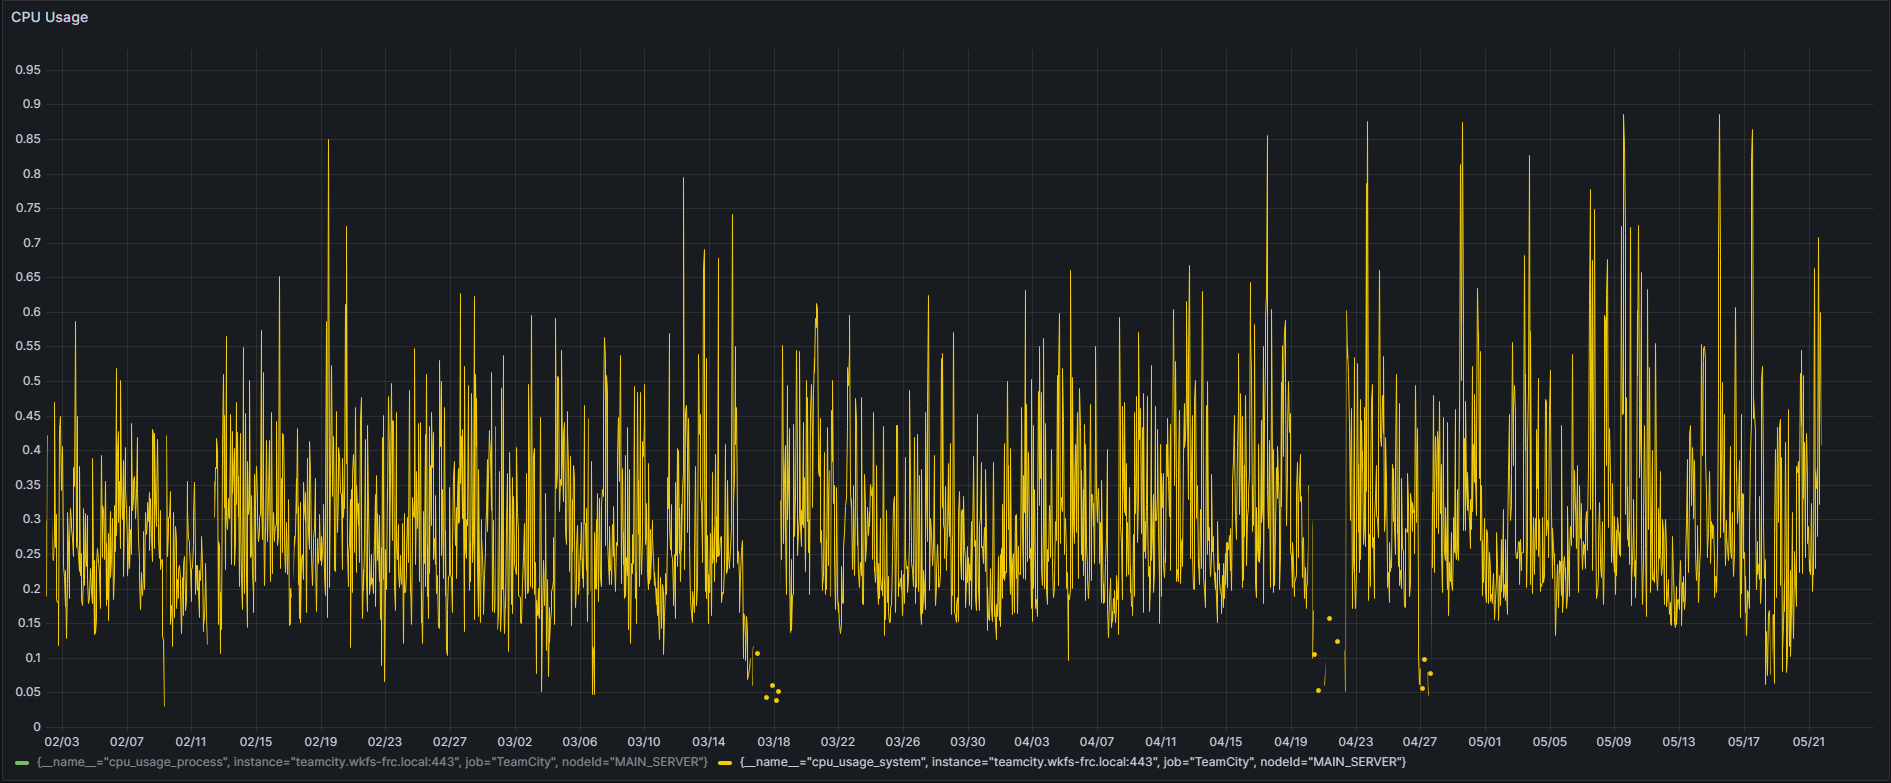
\includegraphics[width=\textwidth]{graphics/cpu.png}
    \caption{CPU Usage}
    \label{fig:cpu}
\end{figure}

\section{Memory Usage}%
\label{sec:memory-usage}

The memory usage is shown in figure \ref{fig:memory}. The green line represents the memory usage of the Eden Space. In the Eden Space new objects are allocated. The yellow line represents the memory usage of the Old Gen, it is where long living objects are stored. We can see a decrease especially in the Old Gen memory usage. 

\begin{figure}[htbp]
    \centering
    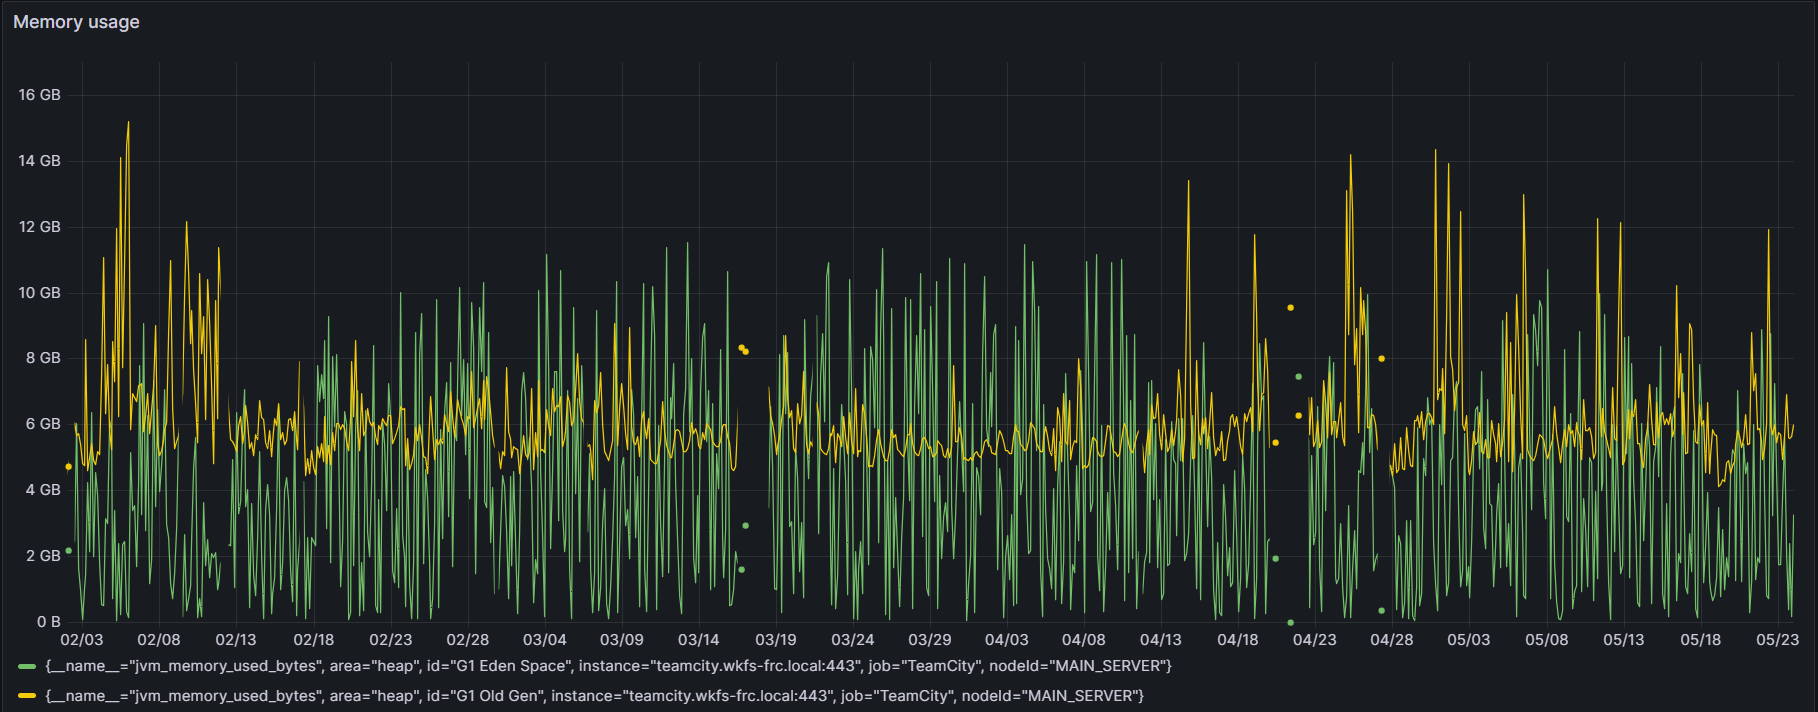
\includegraphics[width=\textwidth]{graphics/memory.png}
    \caption{Memory Usage}
    \label{fig:memory}
\end{figure}

\section{Build Metrics}%
\label{sec:build-metrics}

The amount of builds running at the same time is shown in figure \ref{fig:builds}. There isn't that much difference in the amount of builds running at the same time.

\begin{figure}[htbp]
    \centering
    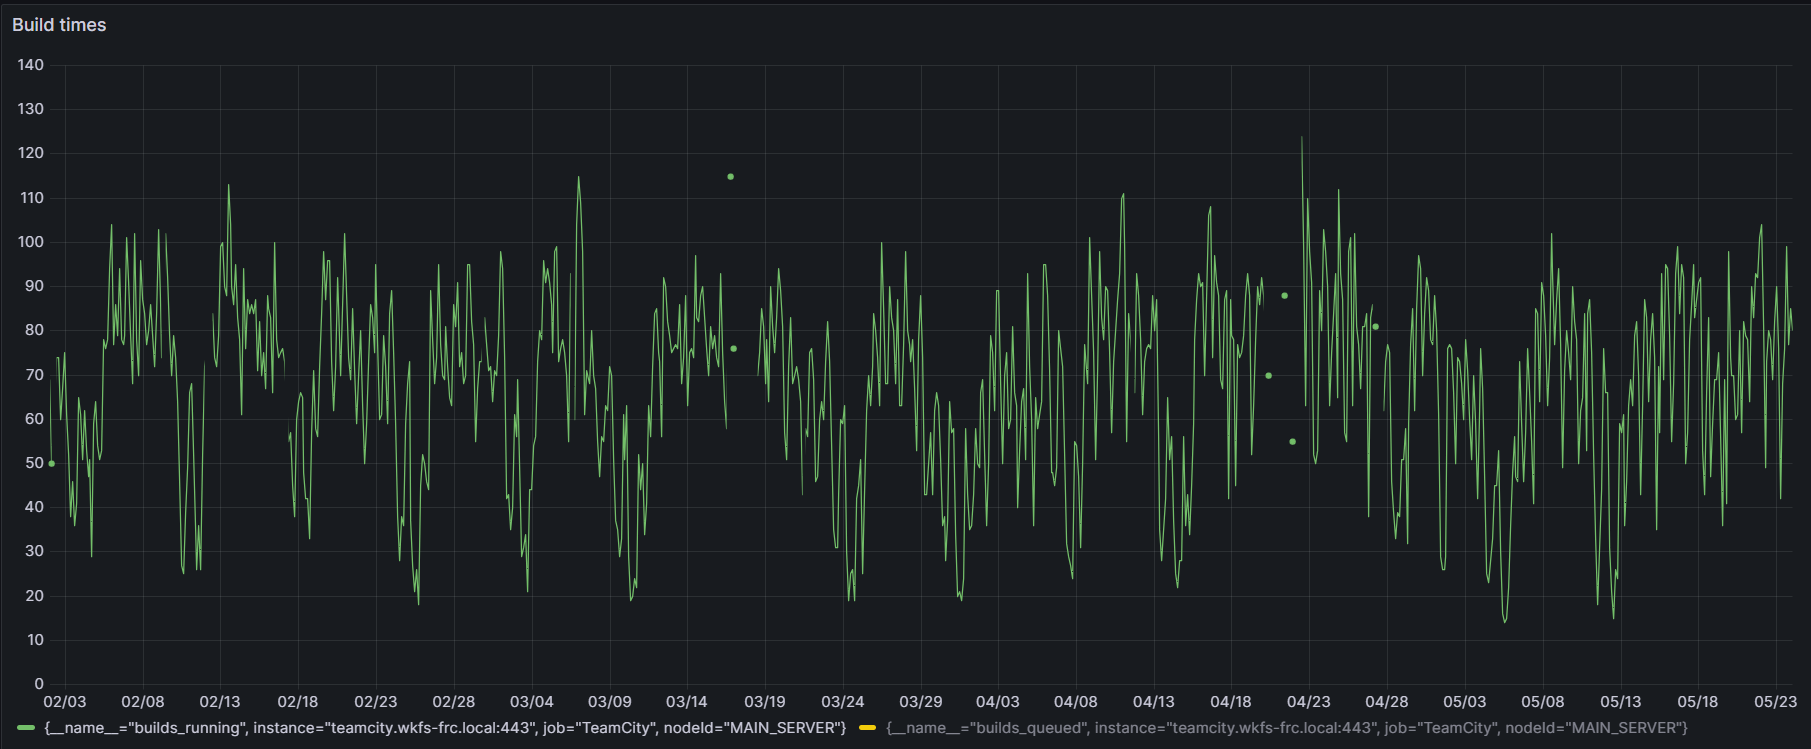
\includegraphics[width=\textwidth]{graphics/builds running.png}
    \caption{Builds running at the same time}
    \label{fig:builds-running}
\end{figure}

The amount of queued builds at the same time is shown in figure \ref{fig:queued-builds}. The average decreased a little bit but there are still some peaks.

\begin{figure}[htbp]
    \centering
    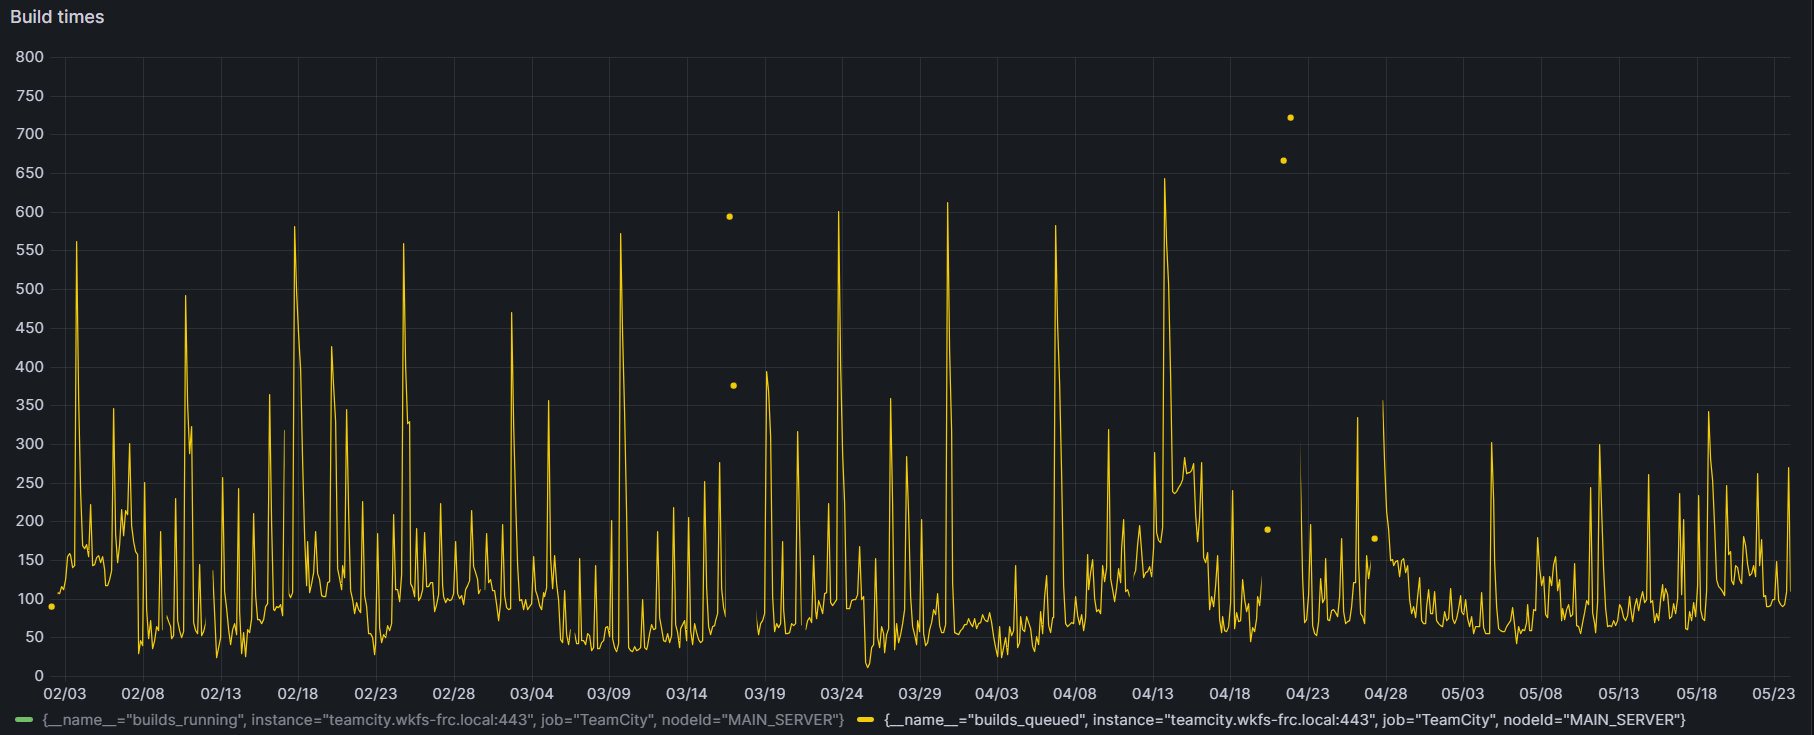
\includegraphics[width=\textwidth]{graphics/builds queued.png}
    \caption{Queued builds}
    \label{fig:queued-builds}
\end{figure}

\section{Resource Utilization}%
\label{sec:resource-utilization}

The amount of database connections is shown in figure \ref{fig:db-connections}. The amount of database connections decreased a lot after the clean-up of the CI/CD pipeline.
This leads to a lower power consumption, but also lower operating costs and a reduced wear and tear of the hardware.

\begin{figure}[htbp]
    \centering
    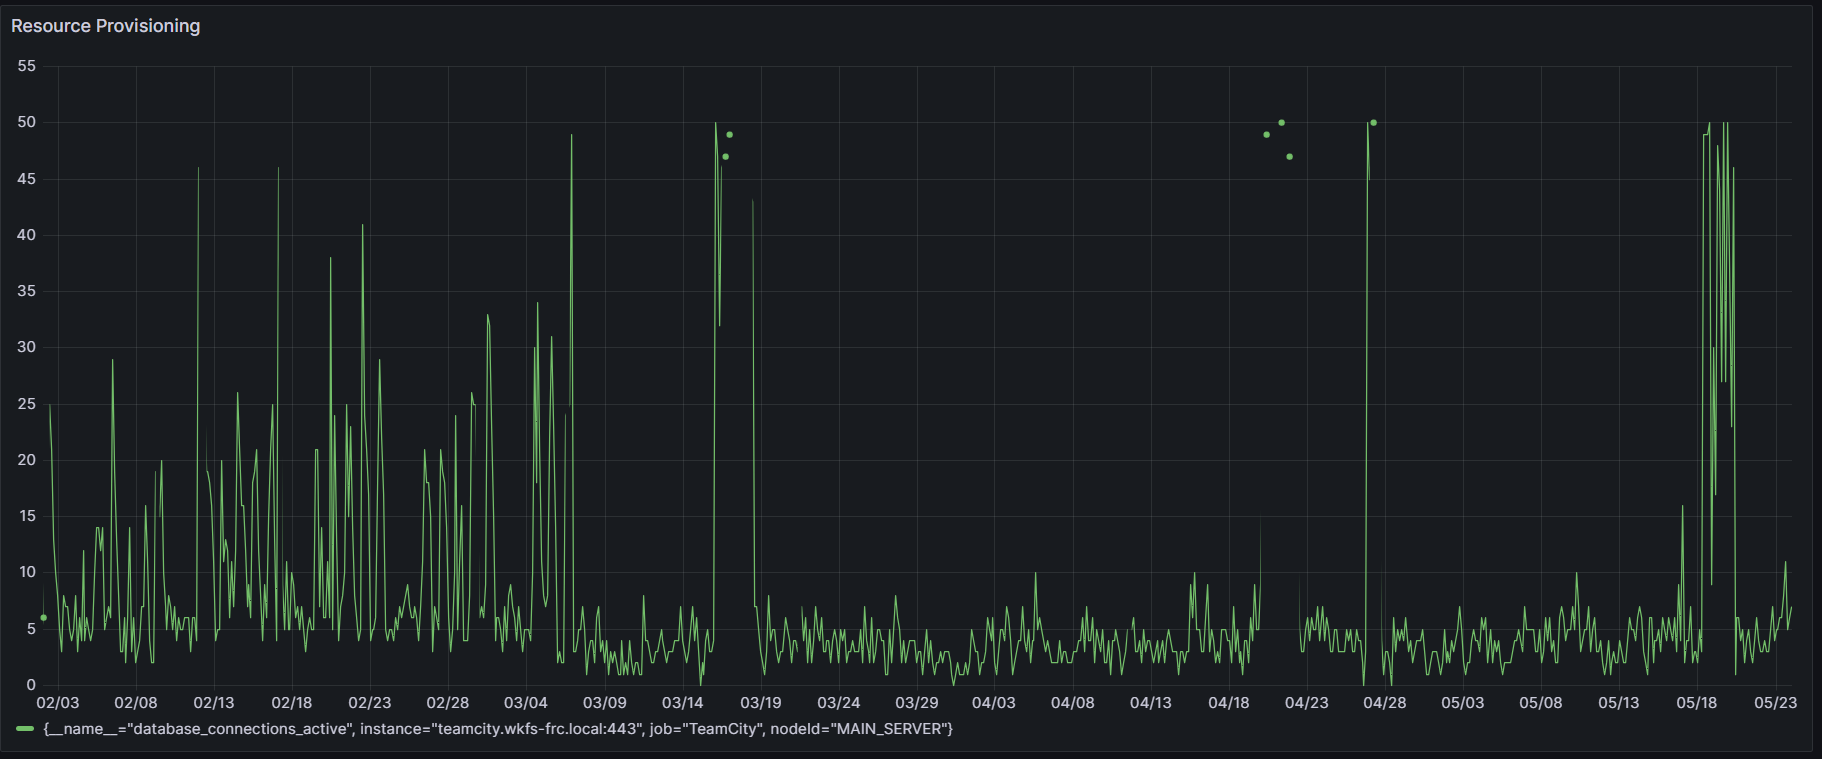
\includegraphics[width=\textwidth]{graphics/DB connections.png}
    \caption{Database connections}
    \label{fig:db-connections}
\end{figure}

\section{Infrastructure scalability}%
\label{sec:infrastructure-scalability}

The amount of agents connected is shown in figure \ref{fig:agents-connected}. 
The amount of agents connected decreased a little bit after the clean-up of the CI/CD pipeline. 
This leads to a lower power consumption, but also lower operating costs and a reduced wear and tear of the hardware.

\begin{figure}[htbp]
    \centering
    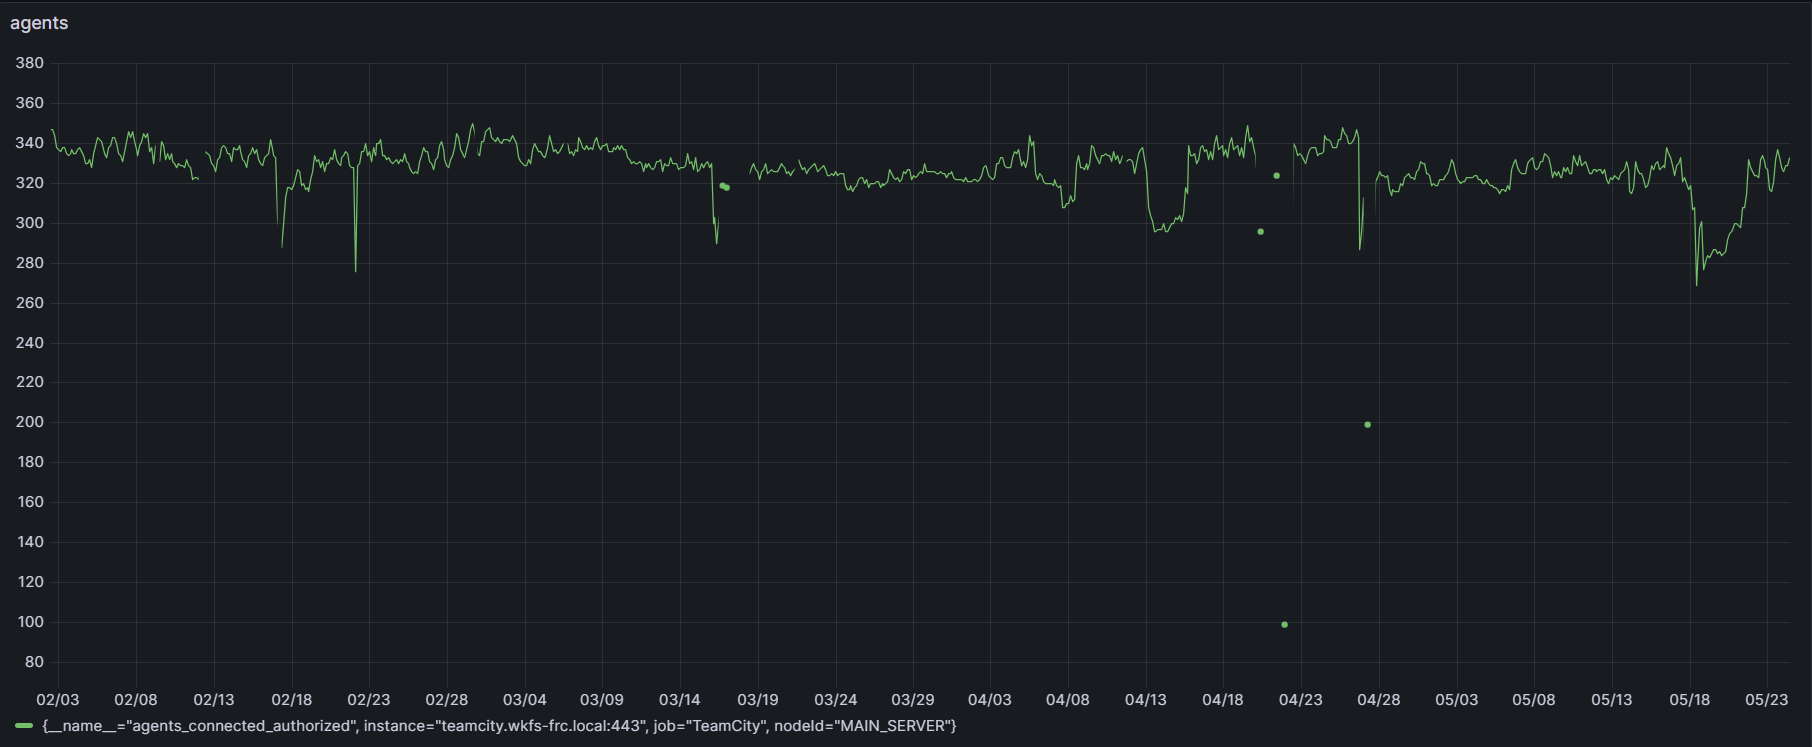
\includegraphics[width=\textwidth]{graphics/agents.png}
    \caption{Agents connected}
    \label{fig:agents-connected}
\end{figure}
%%=============================================================================
%% Conclusie
%%=============================================================================

\chapter{Conclusie}%
\label{ch:conclusie}

% TODO: Trek een duidelijke conclusie, in de vorm van een antwoord op de
% onderzoeksvra(a)g(en). Wat was jouw bijdrage aan het onderzoeksdomein en
% hoe biedt dit meerwaarde aan het vakgebied/doelgroep? 
% Reflecteer kritisch over het resultaat. In Engelse teksten wordt deze sectie
% ``Discussion'' genoemd. Had je deze uitkomst verwacht? Zijn er zaken die nog
% niet duidelijk zijn?
% Heeft het onderzoek geleid tot nieuwe vragen die uitnodigen tot verder 
%onderzoek?

\lipsum[76-80]



%---------- Bijlagen -----------------------------------------------------------

\appendix

\chapter{Onderzoeksvoorstel}

Het onderwerp van deze bachelorproef is gebaseerd op een onderzoeksvoorstel dat vooraf werd beoordeeld door de promotor. Dat voorstel is opgenomen in deze bijlage.

%% TODO: 
%\section*{Samenvatting}

% Kopieer en plak hier de samenvatting (abstract) van je onderzoeksvoorstel.

With the current global warming and high energy prices, companies are knocking at the door to save on resources. 
This study conducts a comparative analysis, researching existing CI/CD frameworks, and explores strategies for enhancing their eco-friendliness. 
Focusing on the CI/CD infrastructure at Wolters Kluwer, the research evaluates the environmental impact of current processes and proposes innovative approaches to make CI/CD more sustainable. 
Through a proof of concept, the thesis implements and assesses these strategies, aiming to contribute insights into the practical application of green computing principles in the software development life cycle. 
The result will not only offer valuable perspectives for the IT industry but also underline the importance of integrating environmental considerations into the core of CI/CD practices for a more sustainable technological future.


% Verwijzing naar het bestand met de inhoud van het onderzoeksvoorstel
%---------- Inleiding ---------------------------------------------------------

% TODO: Is dit voorstel gebaseerd op een paper van Research Methods die je
% vorig jaar hebt ingediend? Heb je daarbij eventueel samengewerkt met een
% andere student?
% Zo ja, haal dan de tekst hieronder uit commentaar en pas aan.

%\paragraph{Opmerking}

% Dit voorstel is gebaseerd op het onderzoeksvoorstel dat werd geschreven in het
% kader van het vak Research Methods dat ik (vorig/dit) academiejaar heb
% uitgewerkt (met medesturent VOORNAAM NAAM als mede-auteur).
% 

\section{Inleiding}%
\label{sec:inleiding}

Waarover zal je bachelorproef gaan? Introduceer het thema en zorg dat volgende zaken zeker duidelijk aanwezig zijn:

\begin{itemize}
  \item kaderen thema
  \item de doelgroep
  \item de probleemstelling en (centrale) onderzoeksvraag
  \item de onderzoeksdoelstelling
\end{itemize}

Denk er aan: een typische bachelorproef is \textit{toegepast onderzoek}, wat betekent dat je start vanuit een concrete probleemsituatie in bedrijfscontext, een \textbf{casus}. Het is belangrijk om je onderwerp goed af te bakenen: je gaat voor die \textit{ene specifieke probleemsituatie} op zoek naar een goede oplossing, op basis van de huidige kennis in het vakgebied.

De doelgroep moet ook concreet en duidelijk zijn, dus geen algemene of vaag gedefinieerde groepen zoals \emph{bedrijven}, \emph{developers}, \emph{Vlamingen}, enz. Je richt je in elk geval op it-professionals, een bachelorproef is geen populariserende tekst. Eén specifiek bedrijf (die te maken hebben met een concrete probleemsituatie) is dus beter dan \emph{bedrijven} in het algemeen.

Formuleer duidelijk de onderzoeksvraag! De begeleiders lezen nog steeds te veel voorstellen waarin we geen onderzoeksvraag terugvinden.

Schrijf ook iets over de doelstelling. Wat zie je als het concrete eindresultaat van je onderzoek, naast de uitgeschreven scriptie? Is het een proof-of-concept, een rapport met aanbevelingen, \ldots Met welk eindresultaat kan je je bachelorproef als een succes beschouwen?

%---------- Stand van zaken ---------------------------------------------------

\section{Literatuurstudie}%
\label{sec:literatuurstudie}

Hier beschrijf je de \emph{state-of-the-art} rondom je gekozen onderzoeksdomein, d.w.z.\ een inleidende, doorlopende tekst over het onderzoeksdomein van je bachelorproef. Je steunt daarbij heel sterk op de professionele \emph{vakliteratuur}, en niet zozeer op populariserende teksten voor een breed publiek. Wat is de huidige stand van zaken in dit domein, en wat zijn nog eventuele open vragen (die misschien de aanleiding waren tot je onderzoeksvraag!)?

Je mag de titel van deze sectie ook aanpassen (literatuurstudie, stand van zaken, enz.). Zijn er al gelijkaardige onderzoeken gevoerd? Wat concluderen ze? Wat is het verschil met jouw onderzoek?

Verwijs bij elke introductie van een term of bewering over het domein naar de vakliteratuur, bijvoorbeeld~\autocite{Hykes2013}! Denk zeker goed na welke werken je refereert en waarom.

Draag zorg voor correcte literatuurverwijzingen! Een bronvermelding hoort thuis \emph{binnen} de zin waar je je op die bron baseert, dus niet er buiten! Maak meteen een verwijzing als je gebruik maakt van een bron. Doe dit dus \emph{niet} aan het einde van een lange paragraaf. Baseer nooit teveel aansluitende tekst op eenzelfde bron.

Als je informatie over bronnen verzamelt in JabRef, zorg er dan voor dat alle nodige info aanwezig is om de bron terug te vinden (zoals uitvoerig besproken in de lessen Research Methods).

% Voor literatuurverwijzingen zijn er twee belangrijke commando's:
% \autocite{KEY} => (Auteur, jaartal) Gebruik dit als de naam van de auteur
%   geen onderdeel is van de zin.
% \textcite{KEY} => Auteur (jaartal)  Gebruik dit als de auteursnaam wel een
%   functie heeft in de zin (bv. ``Uit onderzoek door Doll & Hill (1954) bleek
%   ...'')

Je mag deze sectie nog verder onderverdelen in subsecties als dit de structuur van de tekst kan verduidelijken.

%---------- Methodologie ------------------------------------------------------
\section{Methodologie}%
\label{sec:methodologie}

Hier beschrijf je hoe je van plan bent het onderzoek te voeren. Welke onderzoekstechniek ga je toepassen om elk van je onderzoeksvragen te beantwoorden? Gebruik je hiervoor literatuurstudie, interviews met belanghebbenden (bv.~voor requirements-analyse), experimenten, simulaties, vergelijkende studie, risico-analyse, PoC, \ldots?

Valt je onderwerp onder één van de typische soorten bachelorproeven die besproken zijn in de lessen Research Methods (bv.\ vergelijkende studie of risico-analyse)? Zorg er dan ook voor dat we duidelijk de verschillende stappen terug vinden die we verwachten in dit soort onderzoek!

Vermijd onderzoekstechnieken die geen objectieve, meetbare resultaten kunnen opleveren. Enquêtes, bijvoorbeeld, zijn voor een bachelorproef informatica meestal \textbf{niet geschikt}. De antwoorden zijn eerder meningen dan feiten en in de praktijk blijkt het ook bijzonder moeilijk om voldoende respondenten te vinden. Studenten die een enquête willen voeren, hebben meestal ook geen goede definitie van de populatie, waardoor ook niet kan aangetoond worden dat eventuele resultaten representatief zijn.

Uit dit onderdeel moet duidelijk naar voor komen dat je bachelorproef ook technisch voldoen\-de diepgang zal bevatten. Het zou niet kloppen als een bachelorproef informatica ook door bv.\ een student marketing zou kunnen uitgevoerd worden.

Je beschrijft ook al welke tools (hardware, software, diensten, \ldots) je denkt hiervoor te gebruiken of te ontwikkelen.

Probeer ook een tijdschatting te maken. Hoe lang zal je met elke fase van je onderzoek bezig zijn en wat zijn de concrete \emph{deliverables} in elke fase?

%---------- Verwachte resultaten ----------------------------------------------
\section{Verwacht resultaat, conclusie}%
\label{sec:verwachte_resultaten}

Hier beschrijf je welke resultaten je verwacht. Als je metingen en simulaties uitvoert, kan je hier al mock-ups maken van de grafieken samen met de verwachte conclusies. Benoem zeker al je assen en de onderdelen van de grafiek die je gaat gebruiken. Dit zorgt ervoor dat je concreet weet welk soort data je moet verzamelen en hoe je die moet meten.

Wat heeft de doelgroep van je onderzoek aan het resultaat? Op welke manier zorgt jouw bachelorproef voor een meerwaarde?

Hier beschrijf je wat je verwacht uit je onderzoek, met de motivatie waarom. Het is \textbf{niet} erg indien uit je onderzoek andere resultaten en conclusies vloeien dan dat je hier beschrijft: het is dan juist interessant om te onderzoeken waarom jouw hypothesen niet overeenkomen met de resultaten.



%%---------- Andere bijlagen --------------------------------------------------
% TODO: Voeg hier eventuele andere bijlagen toe. Bv. als je deze BP voor de
% tweede keer indient, een overzicht van de verbeteringen t.o.v. het origineel.
%\input{...}

%%---------- Backmatter, referentielijst ---------------------------------------

\backmatter{}

\setlength\bibitemsep{2pt} %% Add Some space between the bibliograpy entries
\printbibliography[heading=bibintoc]

\end{document}
